Solve the following boundary value problems using the spectral method.\\
For each problem, (i) write down the expansions of the right hand side
functions as linear combinations of the eigenfunctions; 
(ii) write down the sum for the solution $u$ obtained from the spectral method;
and (iii) produce a plot showing the sum of the first twenty terms in the series for $u$.

For parts~(c)--(e) you may use the eigenvalues and eigenfunctions
computed in Problem~1(d) of Problem Set~5, and the results of Section~5.2.3
of the text.  

\begin{enumerate}
\item $\displaystyle{-{d^2 u \over dx^2}(x) = e^x}$, 
      \quad $u(0) = 1$, $u(1) = 0$.\\[0.25em]
\item $\displaystyle{-{d^2 u \over dx^2}(x) - 10 u(x) = e^x}$, 
      \quad $u(0) = 0$, $u(1) = 0$.\\[0.25em]
\item $\displaystyle{-{d^2 u \over dx^2}(x) = x + \sin(\pi x)}$, 
      \quad $\displaystyle{u(0) = {du\over dx}(1) = 0.}$ \\[0.25em]
\item $\displaystyle{-{d^2 u \over dx^2}(x) = x + \sin(\pi x)}$, 
      \quad $\displaystyle{u(0) = {du\over dx}(1) = 1.}$ \\[0.25em]
\item $\displaystyle{-{d^2 u \over dx^2}(x) = f(x)}$, 
      \quad $\displaystyle{{du\over dx}(0) = u(1) = 0,}$ 
      where $\displaystyle{f(x) 
             = \left\{ \begin{array}{ll} 1, & 0<x<1/2;\\ 
                                         0, & 1/2<x<1.
                \end{array}\right.}$ \\[0.25em]
      (This $f$ is not continuous; follow the usual procedure and
       see if you obtain a sensible answer.)
       
\end{enumerate}


%%%%%%%%%%%%%%%%%%%%%%%%%%%%%%%%%%%%%%%%%%%%%%%%%%%%%%%%%%%%%%%%%%%%%%%%%%%%%%%%

\ifthenelse{\boolean{showsols}}{\begin{solution}
\def\uhat{\widehat{u}}
\begin{enumerate}
\item First we solve the problem with homogeneous Dirichlet boundary conditions
using the spectral method, then we will add a correction to satisfy the
inhomogeneous boundary conditions.  

For the operator with homogeneous Dirichlet conditions, 
we have eigenvalues $\lambda_k = k^2 \pi^2$ with associated
(normalized) eigenfunctions $\psi_k(x) = \sqrt{2} \sin(k\pi x)$.
We shall call the solution to the problem with homogeneous Dirichlet conditions 
$\uhat$, which is given by the spectral method
\[ \uhat = \sum_{k=1}^\infty {\ip{f,\psi_k} \over \lambda_k} \psi_k.\]
To compute $\ip{e^x,\psi_k}$, integrate twice by parts to obtain
\begin{eqnarray*}
     \int_0^1 e^x \sqrt{2} \sin(k\pi x) \, d x
       &=& \sqrt{2} \big[e^x \sin(k\pi x) \big]_0^1 
          - {\sqrt{2} \over k\pi} \int_0^1 e^x \cos(k\pi x)\,dx \\[0.5em]
       &=& -{\sqrt{2} \over k\pi} \int_0^1 e^x \cos(k\pi x)\,dx \\[0.5em]
       &=& -{\sqrt{2} \over k\pi} 
           \Big(\big[e^x \cos(k\pi x)\big]_0^1
                   + {1\over k\pi} \int_0^1 e^x \sin(k\pi x)\,dx \Big)\\[0.5em]
       &=& {\sqrt{2}\over k\pi} \big(1-e (-1)^k\big)
                -{\sqrt{2}\over k^2\pi^2} 
                   \int_0^1 e^x \sin(k\pi x)\,dx,
\end{eqnarray*}
from which we discern that
\[\sqrt{2}\Big({1+{1\over k^2\pi^2}}\Big) \int_0^1 e^x \sin(k\pi x)\,dx
        = {\sqrt{2}\over k\pi} (1-(-1)^k e).\]
We conclude that
\[ \ip{f,\psi_k} = \int_0^1 e^x \sqrt{2} \sin(k\pi x) \, d x
              = {\sqrt{2} k\pi \over 1+k^2\pi^2} (1-(-1)^k e).\]
The spectral method thus gives
\[ \uhat = \sum_{k=1}^\infty {\ip{f,\psi_k} \over \lambda_k} \psi_k
         = \sum_{k=1}^\infty {2(1-(-1)^k e)\over k\pi(1+k^2\pi^2)} \sin(k\pi x).\]
Now we need to add some function $w$ to $\uhat$ that will produce a $u = \uhat+w$
that satisfies both the differential equation and the inhomogeneous boundary conditions.
We want
\[ -{d^2 u \over dx^2} = -{d^2 \uhat \over dx^2} - {d^2 w \over dx^2} = e^x,\]
but since we already have
\[ -{d^2 \uhat \over dx^2} = e^x,\]
we need 
\[ -{d^2 w \over dx^2} = 0.\]
In other words, $w$ must be for the form $w(x) = \alpha + \beta x$ for 
some constants $\alpha$ and $\beta$.
Now note that
\[ u(0) = \uhat(0) + w(0) = 0+w(0), \qquad
   u(1) = \uhat(1) + w(1) = 0+w(1), \]
so to satisfy the inhomogeneous conditions we need
\[ w(0) = 1, \qquad w(1) = 0.\]
This is only satisfied if we take $\alpha = 1$, $\beta = -1$.
The final series formula for $u$ is thus
\[ u(x) = 1 - x + \sum_{k=1}^\infty {2(1-(-1)^k e)\over k\pi(1+k^2\pi^2)} \sin(k\pi x).\]

Though it is not asked for in the problem, the exact solution is
\[ u(x) = -e^x+(e-2)x+2.\]
The plots below compare the exact solution to the partial sums involving
$0$, 1, 2, and 20 terms.  The code that produced the plots follows.
\begin{center}
   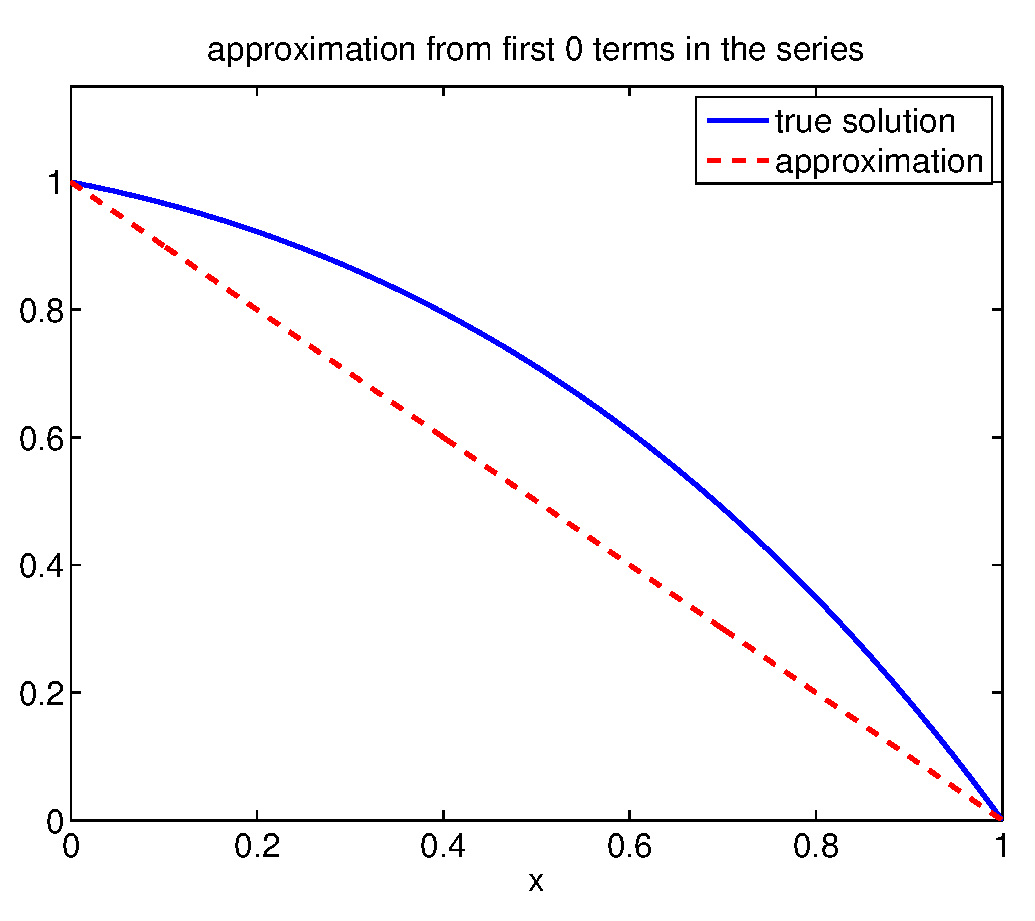
\includegraphics[scale=0.4]{bvps1_0}\quad
   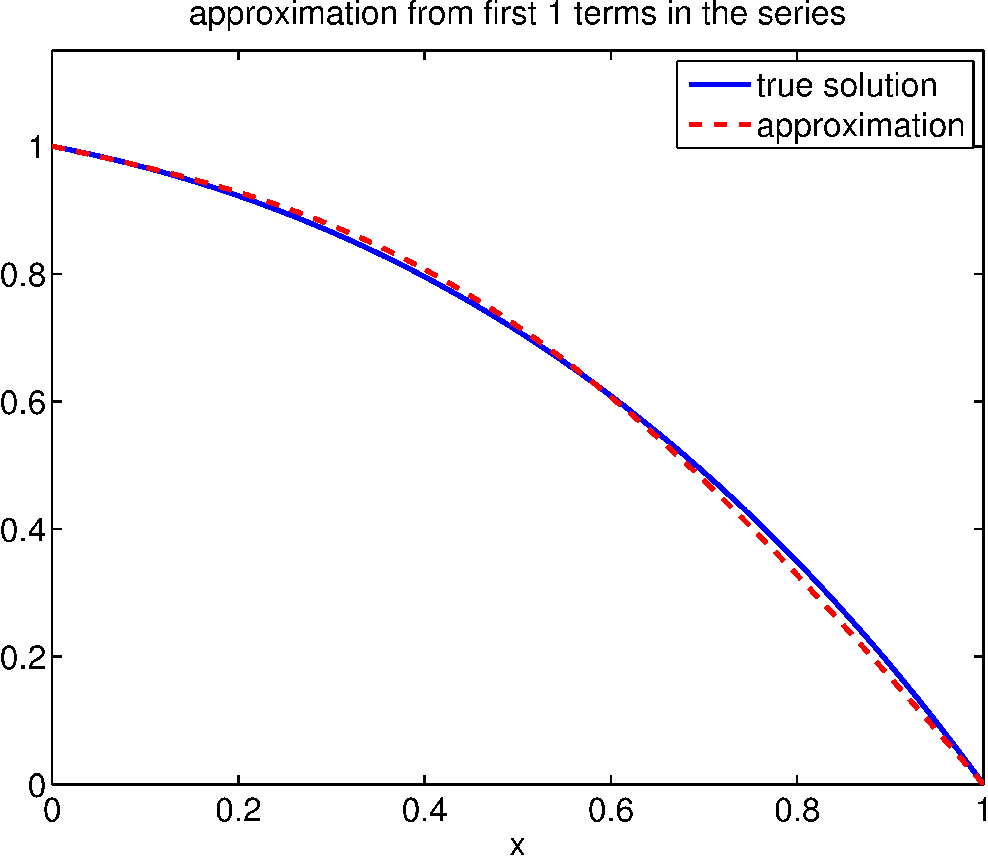
\includegraphics[scale=0.4]{bvps1_1}

   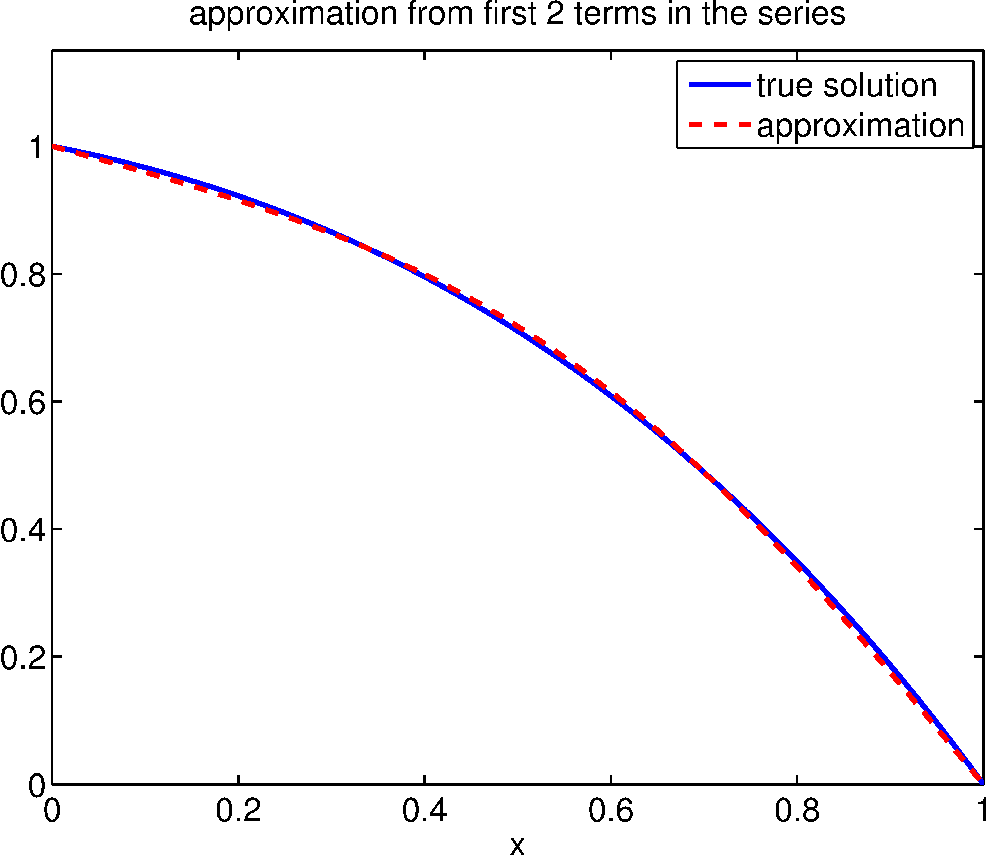
\includegraphics[scale=0.4]{bvps1_2}\quad
   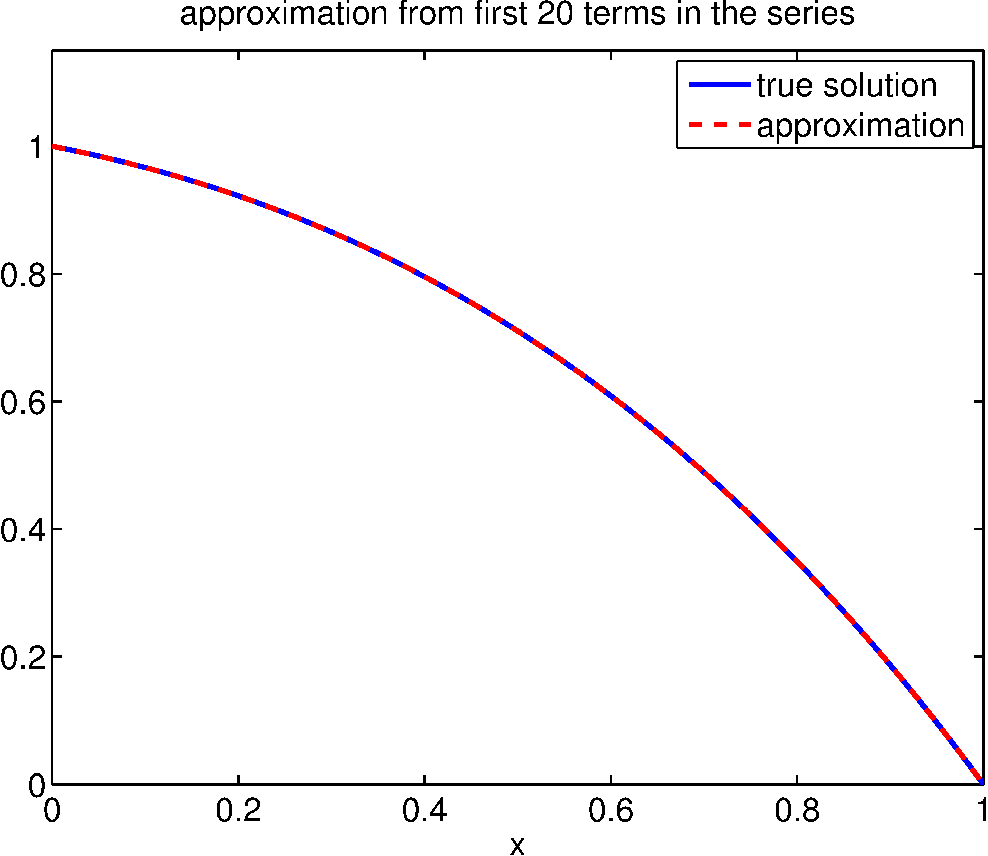
\includegraphics[scale=0.4]{bvps1_20}
\end{center}
\input bvps_code1

%%%%%%%%%%%%%%%%%%%%%%%%%%%%%%%%%%%%%%%%%%%%%%%%%%%%%%%%%%%%%%%%%%%%%%%%%%%%%%%%

\item To solve this problem, identify the linear operator as
\[ L u = -u'' - 10 u,\]
acting the space $C^2_D[0,1]$.  To find the eigenvalues $\lambda_k$ and eigenfunctions $\psi_k$,
notice that $L \psi_k = \lambda_k \psi_k$ is equivalent to
\[ -\psi_k'' - 10 \psi_k = \lambda_k \psi_k,\]
which can be rewritten as
\[ -\psi_k'' = (\lambda_k + 10) \psi_k.\]
Thus, the eigenfunctions $\psi_k$ will be the same as our usual eigenfunctions for $-u''$ on
$C^2_D[0,1]$: 
\[ \psi_k(x) = \sqrt{2} \sin(k \pi x).\]
The eigenvalues must satisfy $\lambda_k + 10 = k^2 \pi^2$, in other words,
\[ \lambda_k = k^2\pi^2 - 10.\]
Now we are prepared to solve the problem using the spectral method.  
Since the right hand side $f(x) = e^x$ is the same as in part~(a), 
and the eigenfunctions are the same, we can simply use the expression
we have already derived:
\[ f(x) = \sum_{k=1}^\infty {\ip{f,\psi_k} \over \ip{\psi_k,\psi_k}} \psi_k
         = \sum_{k=1}^\infty {2(1-(-1)^k e) k \pi \over (1+k^2\pi^2)} \sin(k\pi x).\]
To get the solution $u(x)$, we merely divide each term in the series for $f$ by the eigenvalues:
\[ u(x) = \sum_{k=1}^\infty {\ip{f,\psi_k} \over \ip{\psi_k,\psi_k}} {1\over \lambda_k} \psi_k
         = \sum_{k=1}^\infty {2(1-(-1)^k e) k \pi \over (1+k^2\pi^2)(k^2\pi^2 - 10)} \sin(k\pi x).\]
The plots below compare the exact solution to the partial sums involving
1, 2, and 20 terms, along with the error in the 20-term approximation.  
Code to produce these plots follows.  
The first term in the series gives an excellent approximation!  Why?
Because when $k=1$, the first eigenvalue $\lambda_1 = \pi^2- 10\approx -0.130$ 
is quite a bit smaller than $\lambda_2 = 4\pi^2 - 10 \approx 29.478$, so 
the first term is quite a bit larger than the next one.
\begin{center}
   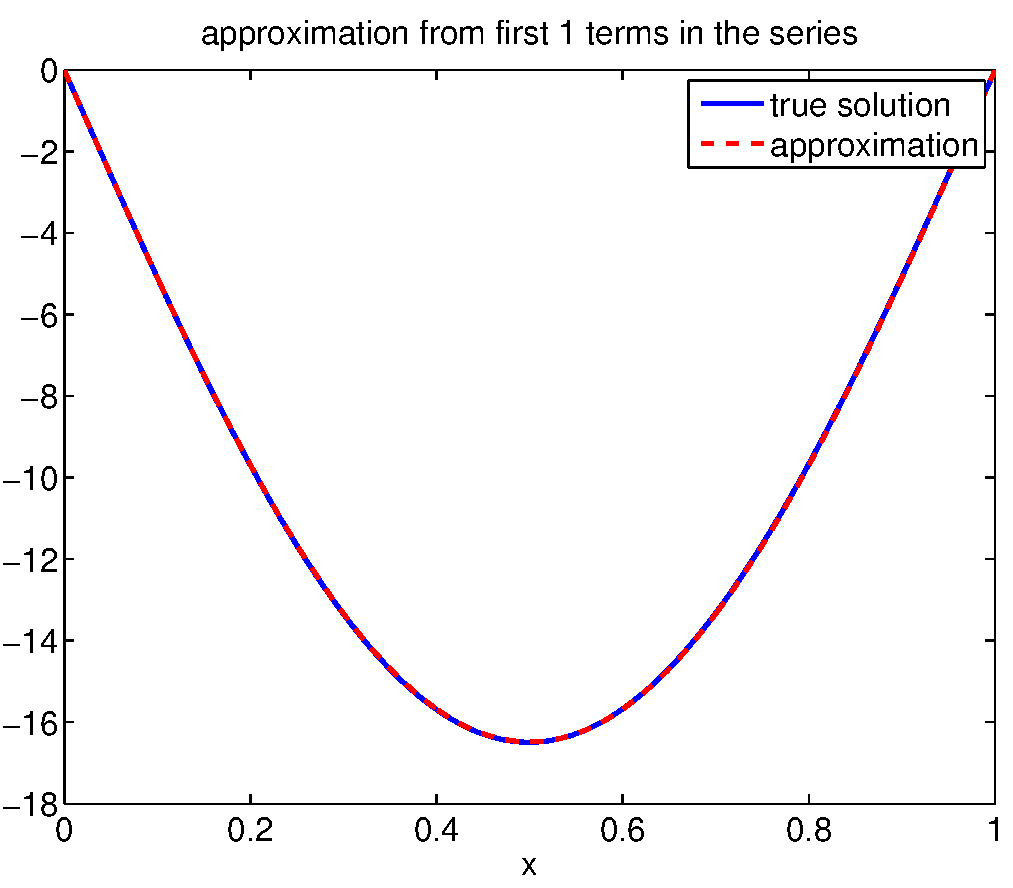
\includegraphics[scale=0.4]{bvps4_1}\quad
   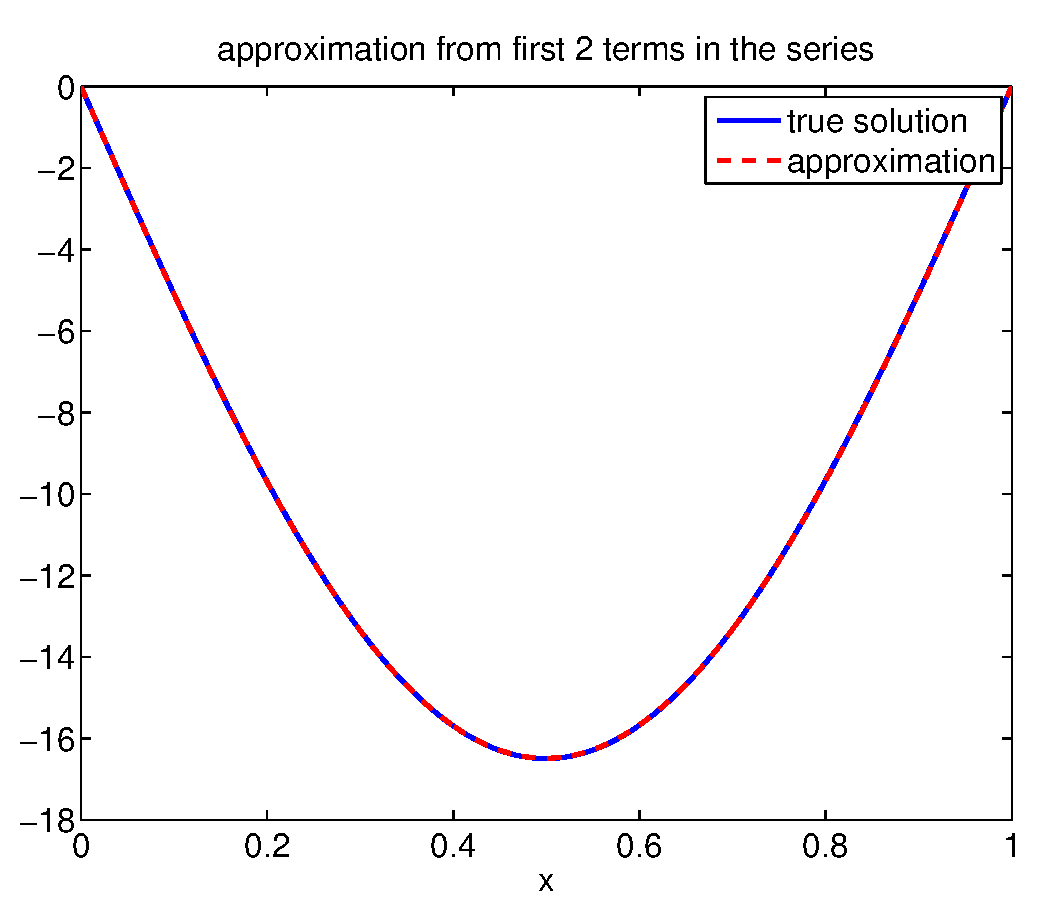
\includegraphics[scale=0.4]{bvps4_2}

   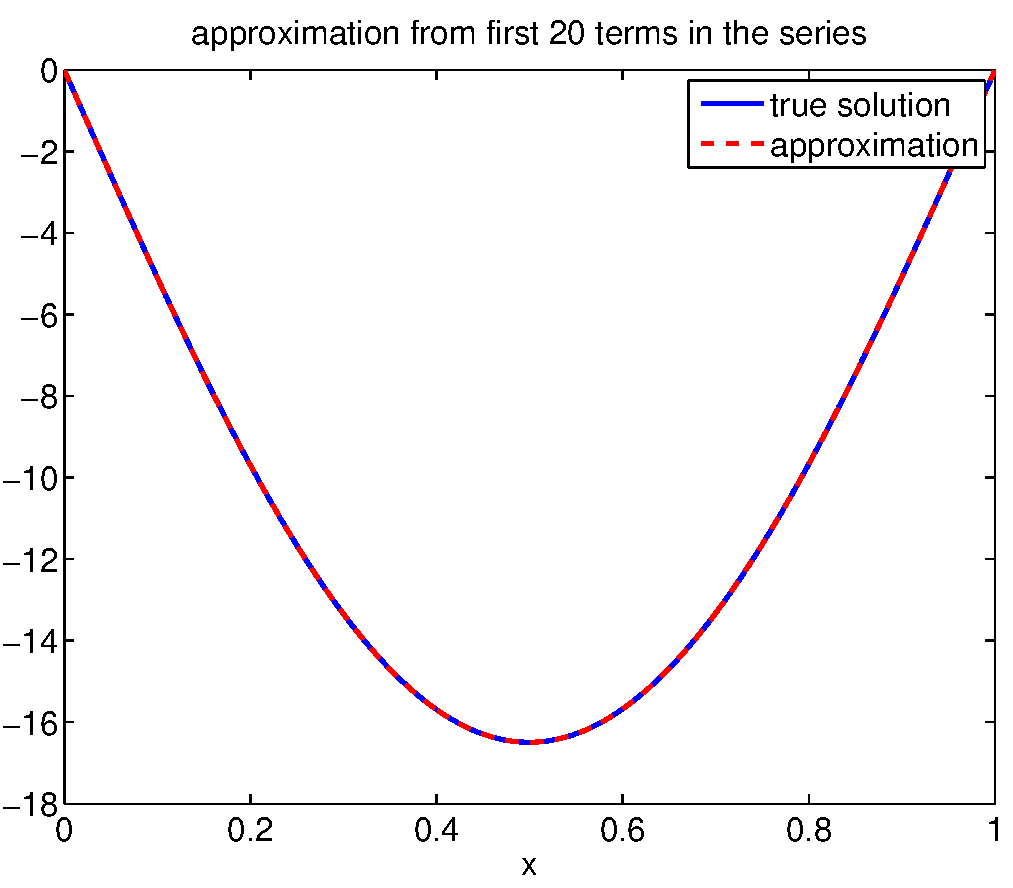
\includegraphics[scale=0.4]{bvps4_20}\quad
   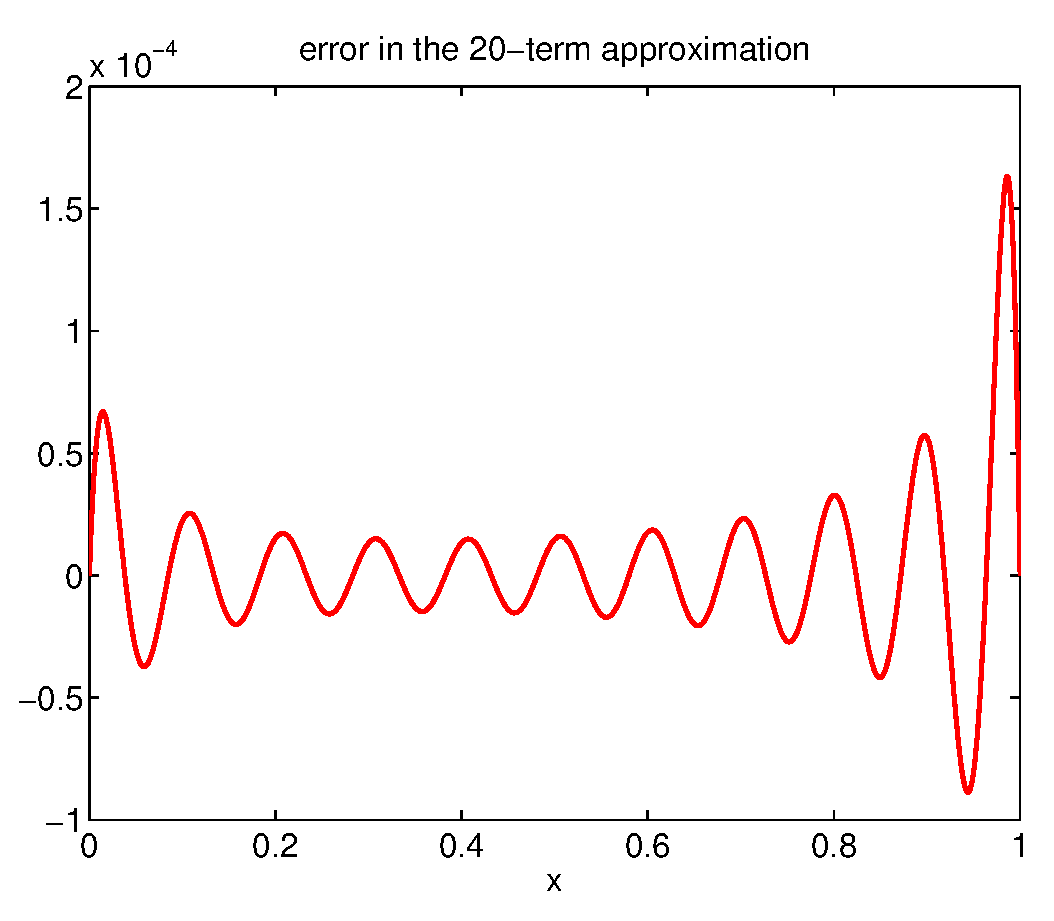
\includegraphics[scale=0.4]{bvps4_20_err}
\end{center}
\input bvps_code1



%%%%%%%%%%%%%%%%%%%%%%%%%%%%%%%%%%%%%%%%%%%%%%%%%%%%%%%%%%%%%%%%%%%%%%%%%%%%%%%%

 \item One can readily compute (or look up in the textbook) 
      the eigenvalues and (orthonormal) eigenfunctions for these boundary conditions:
     \begin{eqnarray*} \lambda_k &=& (k-1/2)^2 \pi^2, \quad k = 1, 2, \ldots \\[0.5em]
                        \psi_k &=& \sqrt{2} \sin(\sqrt{\lambda_k} x).
      \end{eqnarray*}
     We now need to compute the inner products $\ip{x+\sin(\pi x), \psi_k}$, which we can do
     in pieces:
     \begin{eqnarray*} 
          \ip{x, \psi_k} &=& \sqrt{2} \int_0^1 x \sin(\sqrt{\lambda_k} x) \, dx  \\[0.5em]
                      &=& {\sqrt{2}(\sqrt{\lambda_k}\cos(\sqrt{\lambda_k})+\sin(\sqrt{\lambda_k})
                               \over \lambda_k}
                      = {\sqrt{2}(-1)^{k+1} \over \lambda_k}.
     \end{eqnarray*}
     twice integrating by parts shows that
       \[ \int_0^1 \sin(\alpha x) \sin(\beta)x\, dx
             = {\alpha \cos(\alpha)\sin(\beta) - \beta\sin(\alpha)\cos(\beta) 
                    \over \beta^2-\alpha^2},\]
     and hence
       \[   \ip{\sin(\pi x), \psi_k} = {\sqrt{2} (-1)^k \over ((k-1/2)^2-1)\pi}
                                  = {\sqrt{2} (-1)^k \pi\over (\lambda_k - \pi^2)}.\]
     We put these pieces together to find that
       \[   \ip{x+\sin(\pi x), \psi_k} = 
                  {\sqrt{2}(-1)^{k+1} \over \lambda_k}
                + {\sqrt{2} (-1)^k \pi\over (\lambda_k - \pi^2)}.\]

The spectral method thus gives the formula
\begin{eqnarray*}
     u(x) &=& \sum_{k=1}^\infty 
                  2(-1)^k\Big({\pi\over \lambda_k(\lambda_k - \pi^2)} 
                               - {1\over \lambda_k^2}\Big)
                              \sin(\sqrt{\lambda_k} x) \\[0.5em]
          &=& \sum_{k=1}^\infty 
                   {2 (-1)^k \big((\pi-1)\lambda_k - \pi^2\big)
                     \over \lambda_k^2(\lambda_k-\pi^2)}
                              \sin(\sqrt{\lambda_k} x).
\end{eqnarray*}
The true solution can be determined to be
\[ u(x) = {\sin(\pi x) \over \pi^2} -{x^3 \over 6} + {x\over 2} + {x\over \pi}.\]
The plots below compare the exact solution to the partial sums involving
1, 2, 3, and 20 terms.  The code that produced the plots follows.
\begin{center}
   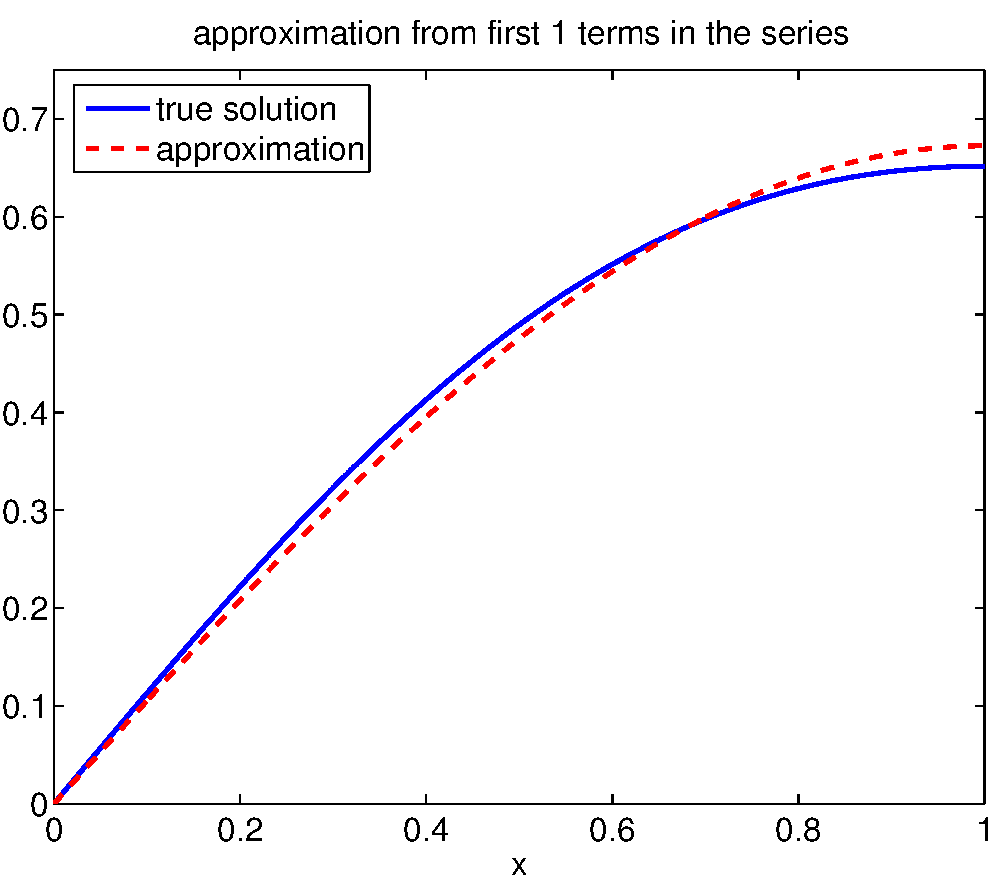
\includegraphics[scale=0.4]{bvps2_1}\quad
   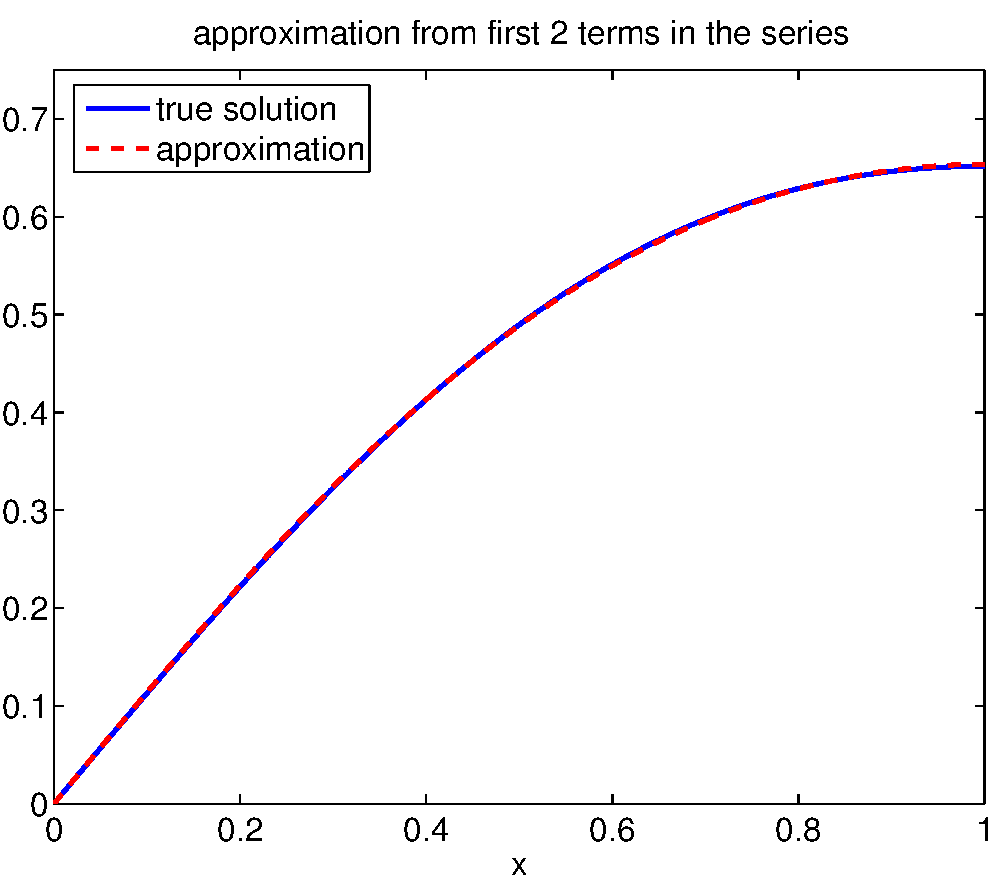
\includegraphics[scale=0.4]{bvps2_2}

   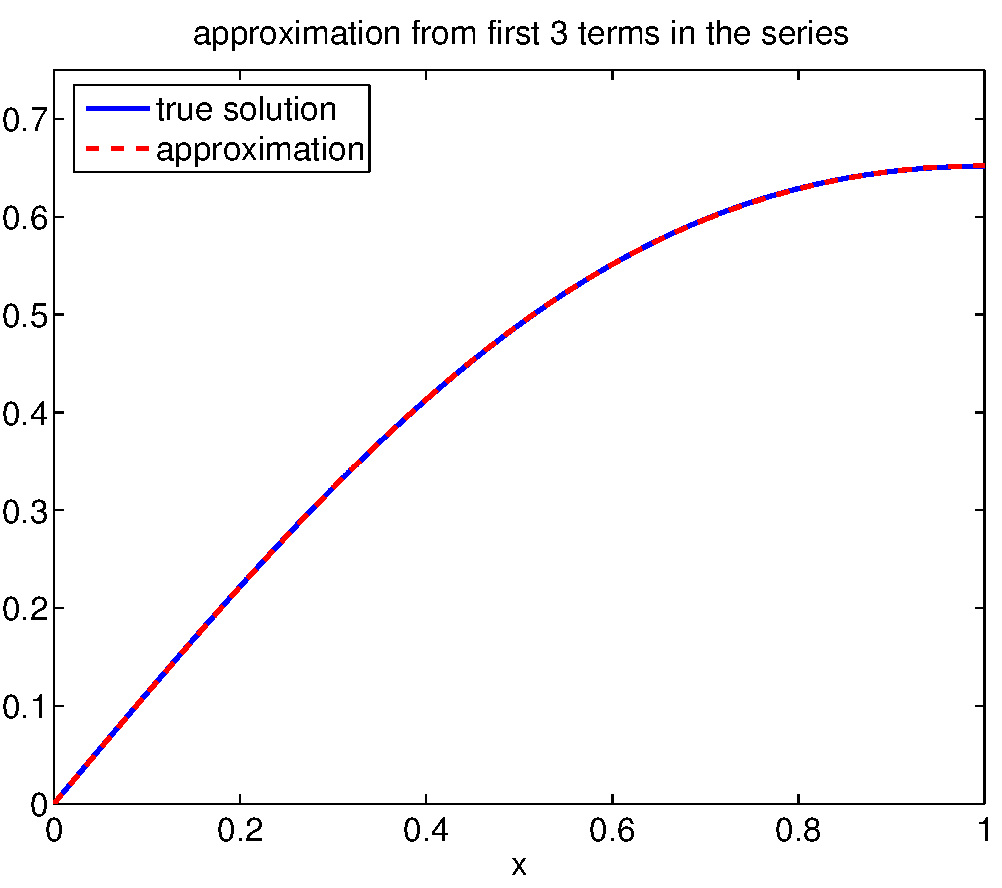
\includegraphics[scale=0.4]{bvps2_3}\quad
   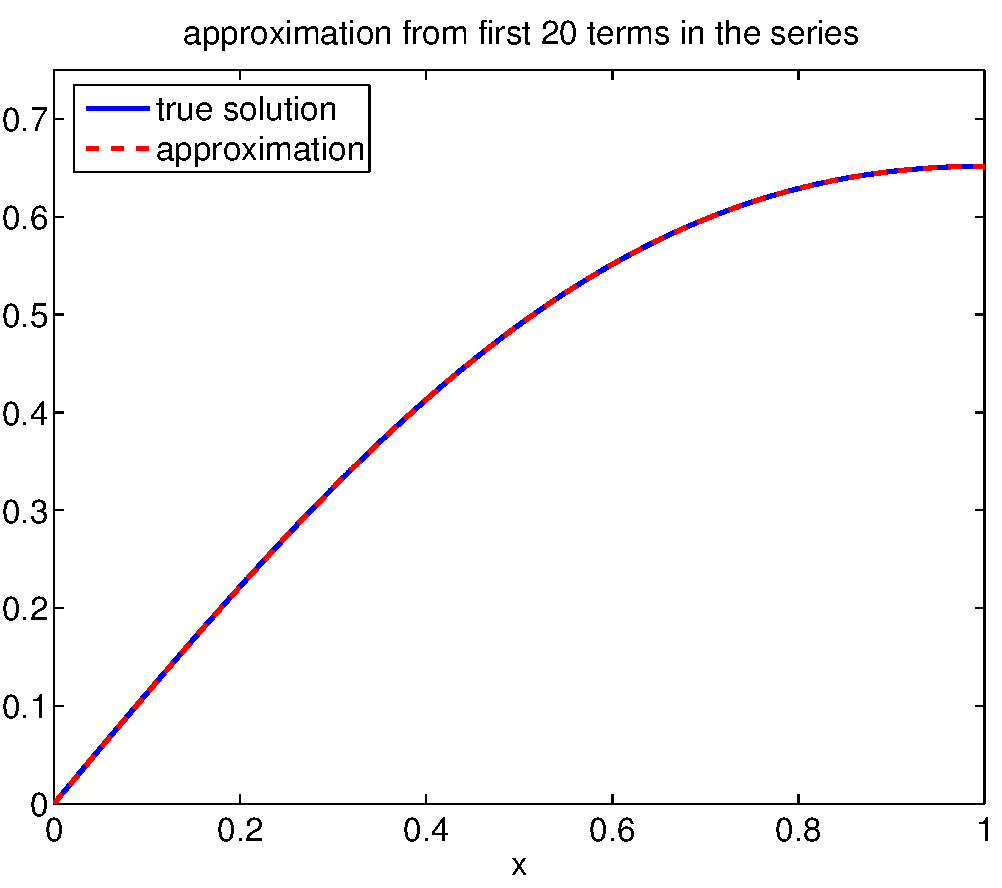
\includegraphics[scale=0.4]{bvps2_20}
\end{center}
\input bvps_code2

\item Notice that this problem is identical to part~(c), except
now with the inhomogeneous boundary conditions $u(0) = u'(1) = 1$.
As in part~(a), we seek a solution $u = \widehat{u} + w$, where
$\widehat{u}$ satisfies the equation with homogeneous boundary conditions
(from part~(c)),
\begin{eqnarray*}
    \widehat{u}(x)
          &=& \sum_{k=1}^\infty 
                   {2 (-1)^k \big((\pi-1)\lambda_k - \pi^2\big)
                     \over \lambda_k^2(\lambda_k-\pi^2)}
                              \sin(\sqrt{\lambda_k} x) \\
          &=& {\sin(\pi x) \over \pi^2} -{x^3 \over 6} + {x\over 2} + {x\over \pi},
\end{eqnarray*}
and $w$ is a function with $-w''(x) = 0$, i.e., $w(x) = \alpha + \beta x$.
In this case we require 
\[ u(0) = \widehat{u}(0) + w(0) = \alpha = 1\]
and 
\[ u'(1) = \widehat{u}'(1) + w'(0) = beta = 1.\]
Hence, the solution is given by
\begin{eqnarray*}
   u(x) &=& 1 + x + 
             \sum_{k=1}^\infty 
                   {2 (-1)^k \big((\pi-1)\lambda_k - \pi^2\big)
                     \over \lambda_k^2(\lambda_k-\pi^2)}
                              \sin(\sqrt{\lambda_k} x) \\
        &=& 1 + x + {\sin(\pi x) \over \pi^2} -{x^3 \over 6} + {x\over 2} + {x\over \pi}.
\end{eqnarray*}
The plots below compare the exact solution to the partial sums involving
1, 2, 3, and 20 terms.  The code that produced the plots follows.
\begin{center}
   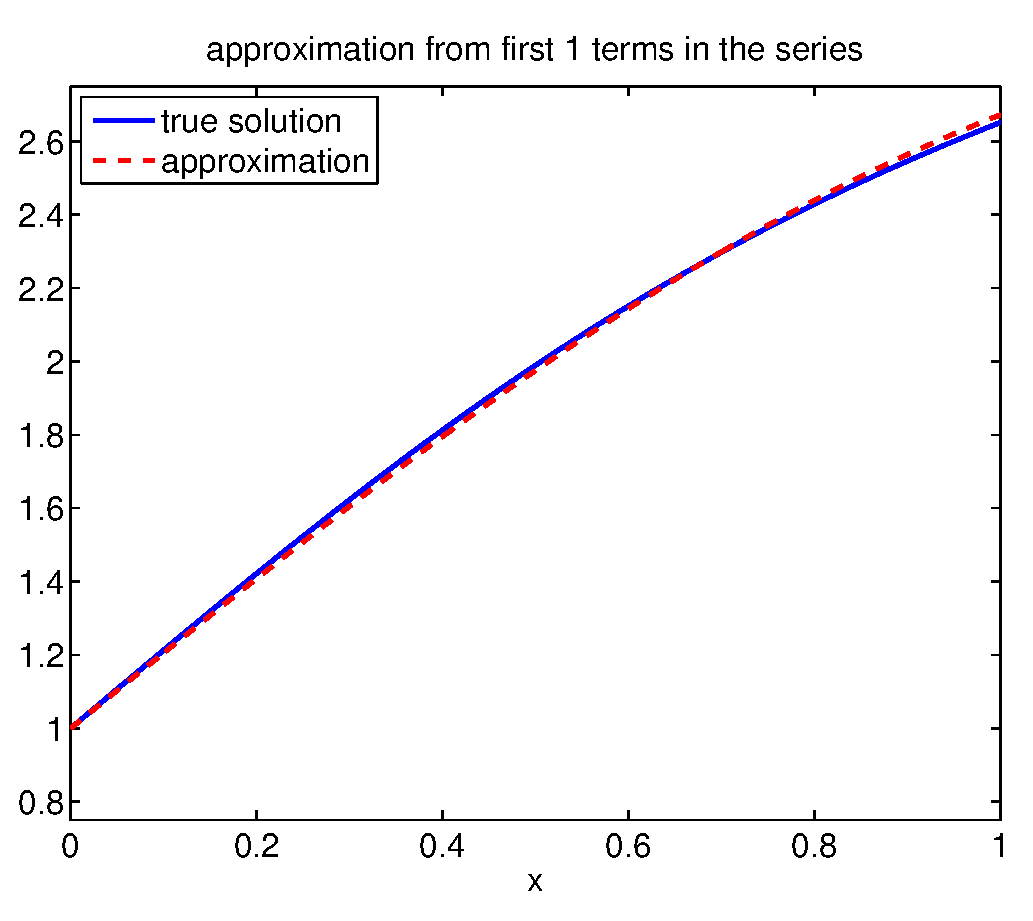
\includegraphics[scale=0.4]{bvps2b_1}\quad
   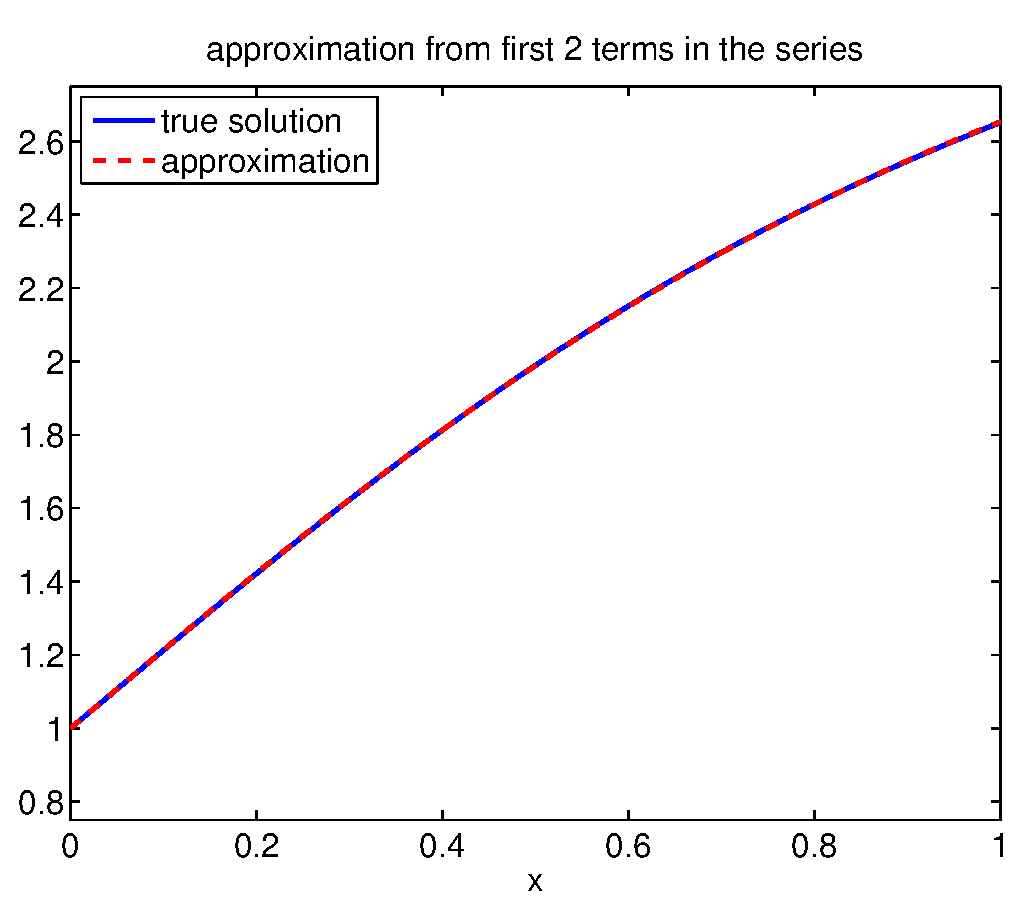
\includegraphics[scale=0.4]{bvps2b_2}

   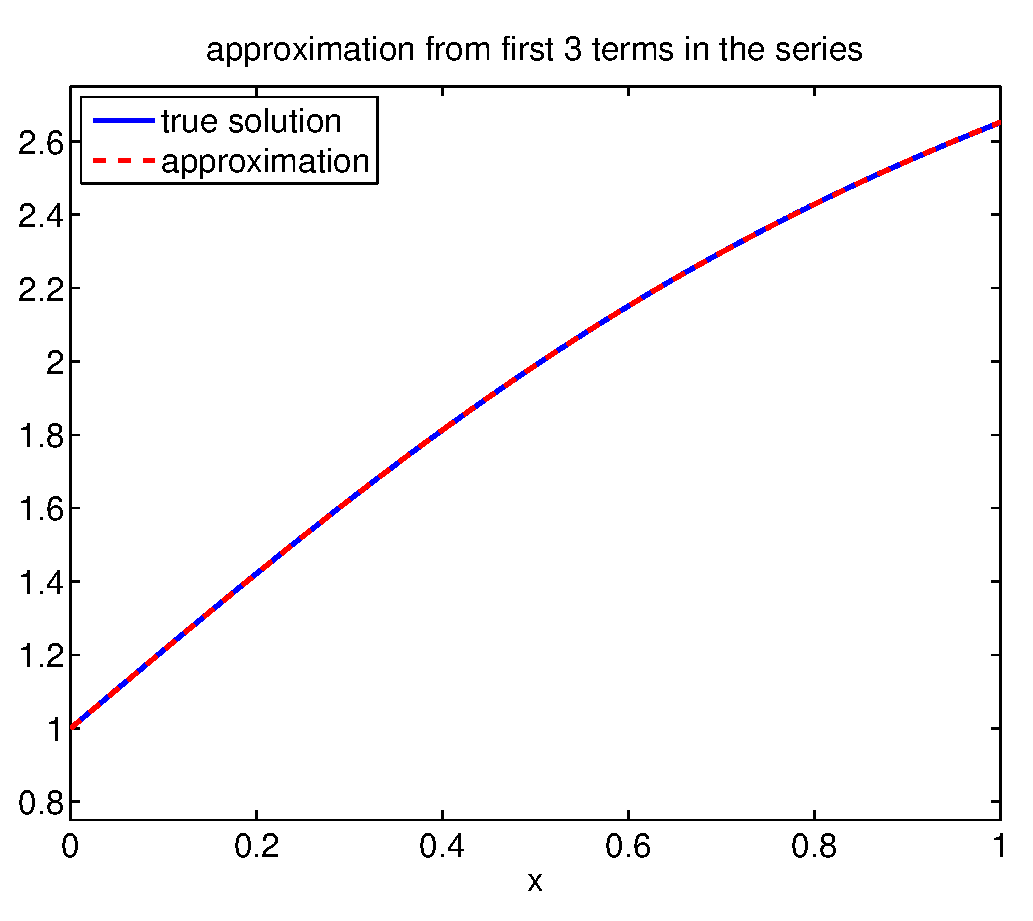
\includegraphics[scale=0.4]{bvps2b_3}\quad
   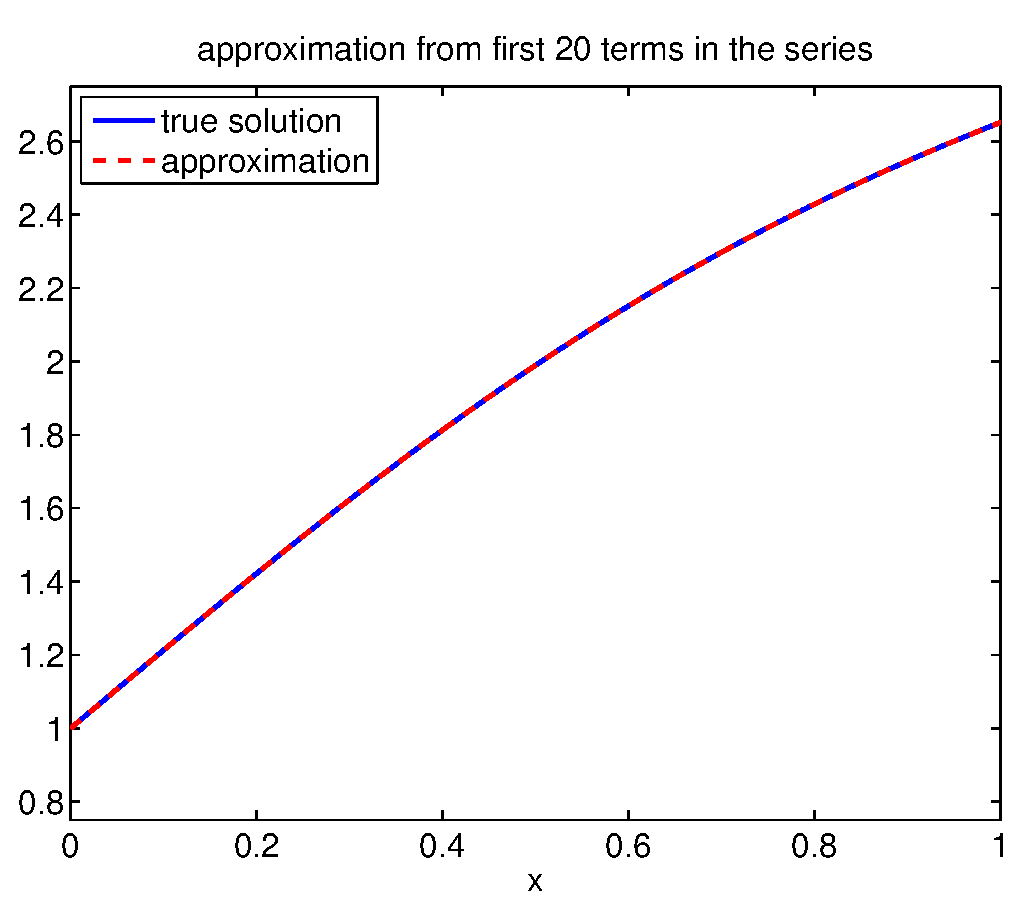
\includegraphics[scale=0.4]{bvps2b_20}
\end{center}
\input bvps_code2b




\item On Problem Set~5, the eigenvalues and eigenfunctions for this example
      were determined to be
     \begin{eqnarray*} \lambda_k &=& (k-1/2)^2 \pi^2, \quad k = 1, 2, \ldots \\[0.5em]
                        \psi_k &=& \sqrt{2} \cos(\lambda_k x).
      \end{eqnarray*}
Though the function $f$ is discontinuous, we proceed as usual, computing
\begin{eqnarray*}
     \ip{f,\psi_k} = \int_0^1 f(x) \psi_k(x)\,dx  
                &=& \int_0^{1/2} \psi_k(x)\,dx \\
                &=& \int_0^{1/2} \sqrt{2}@\cos(\sqrt{\lambda_k} x)\,dx 
                = \sqrt{2}@\Big[{\sin(\sqrt{\lambda_k} x) 
                                   \over \sqrt{\lambda_k}}\Big]_0^{1/2} 
                = {\sqrt{2}@\sin(\sqrt{\lambda_k}/2)\over \sqrt{\lambda_k}}.
\end{eqnarray*}
\textbf{Note the slow decay} of these coefficients, even though $f$ satisfies
the same boundary conditions as the eigenfunctions!  This is due to the 
discontinuity on the interior of the domain, as seen in the following plots.
\begin{center}
   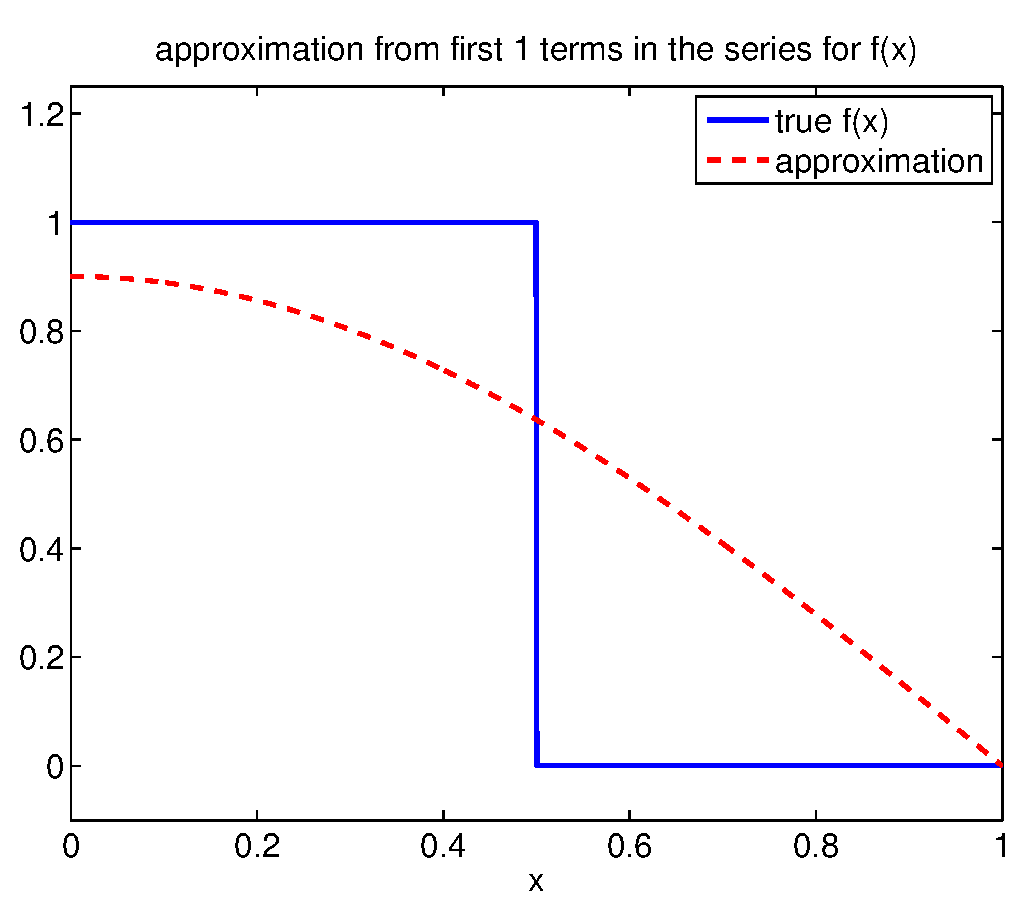
\includegraphics[scale=0.4]{bvps3_1b}\quad
   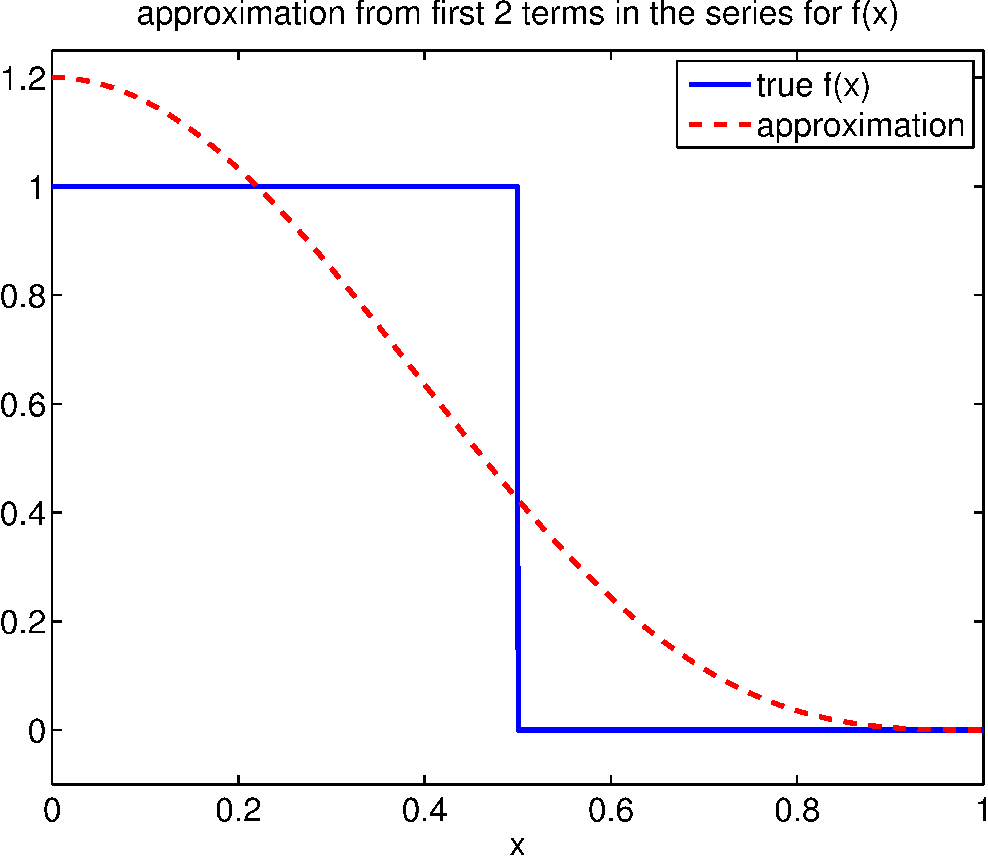
\includegraphics[scale=0.4]{bvps3_2b}

   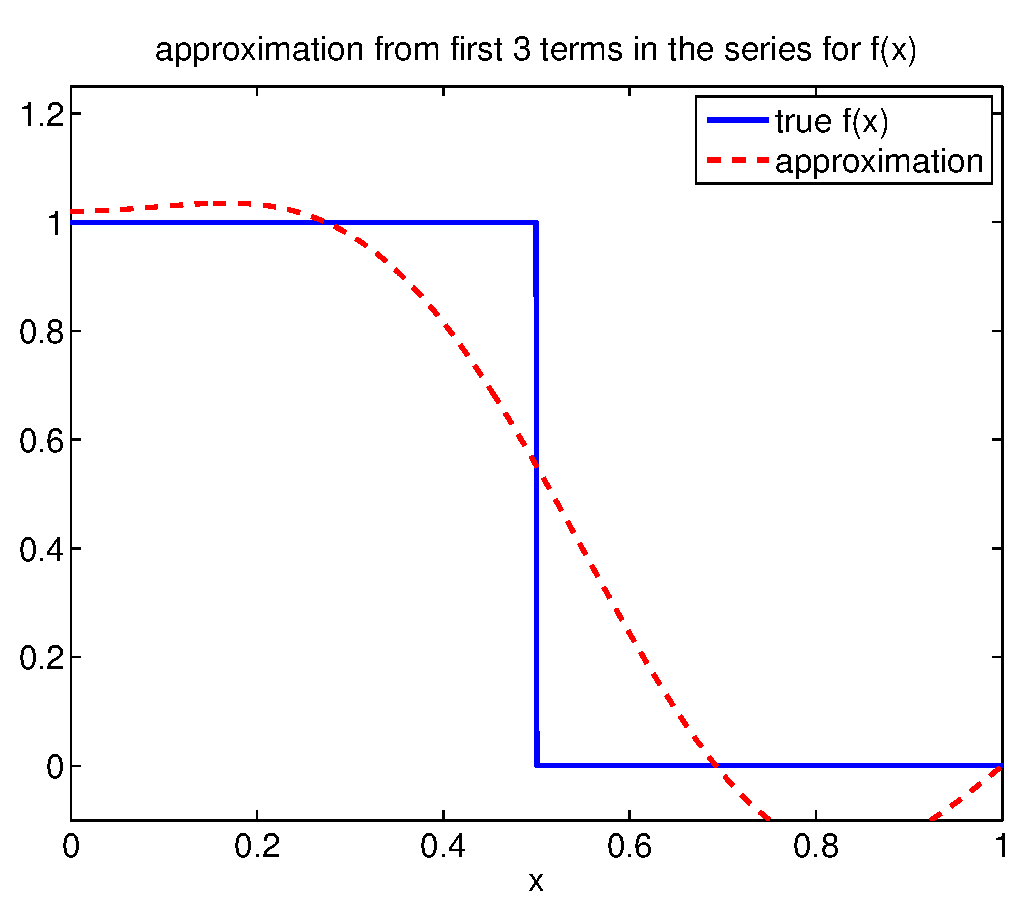
\includegraphics[scale=0.4]{bvps3_3b}\quad
   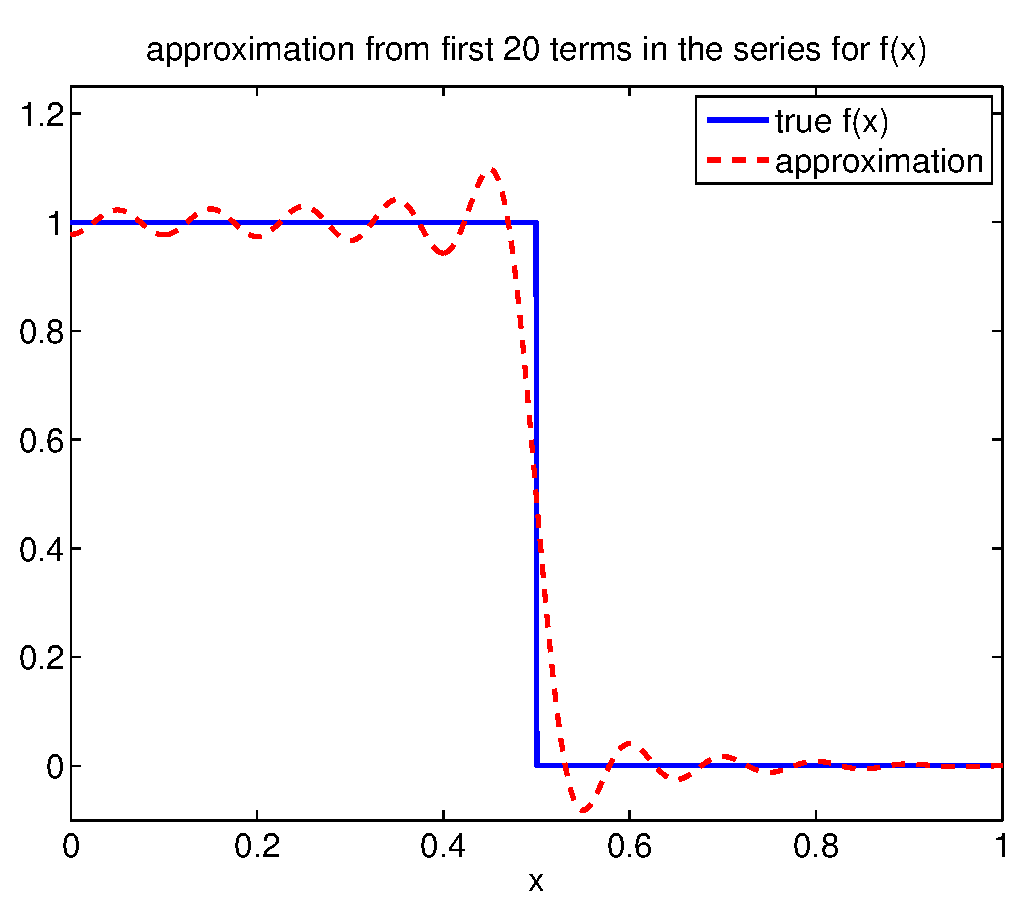
\includegraphics[scale=0.4]{bvps3_20b}
\end{center}

The spectral method thus gives the solution as the formula
\[ u(x) = \sum_{k=0}^\infty = {2 \sin(\sqrt{\lambda_k}/2) \over \lambda_k^{3/2}}
                                 \cos(\sqrt{\lambda_k} x).\]
The plots below show the partial sums involving
1, 2, 3, and 20 terms.  The code that produced the plots follows.
\begin{center}
   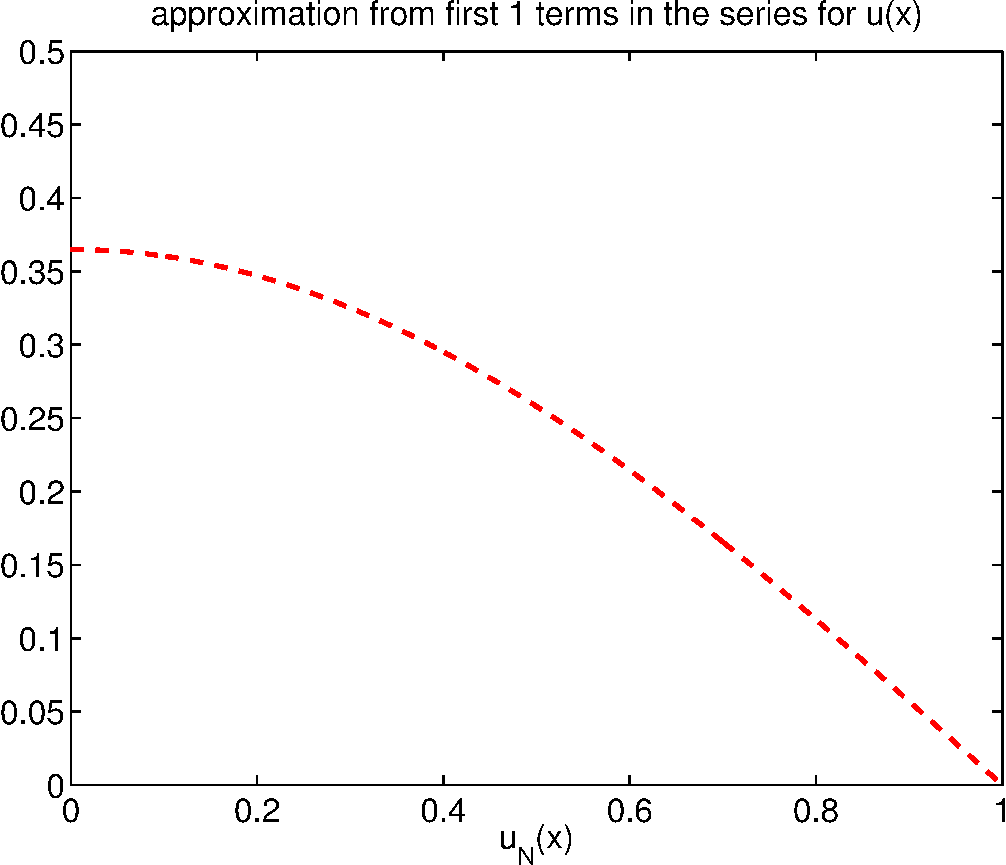
\includegraphics[scale=0.4]{bvps3_1a}\quad
   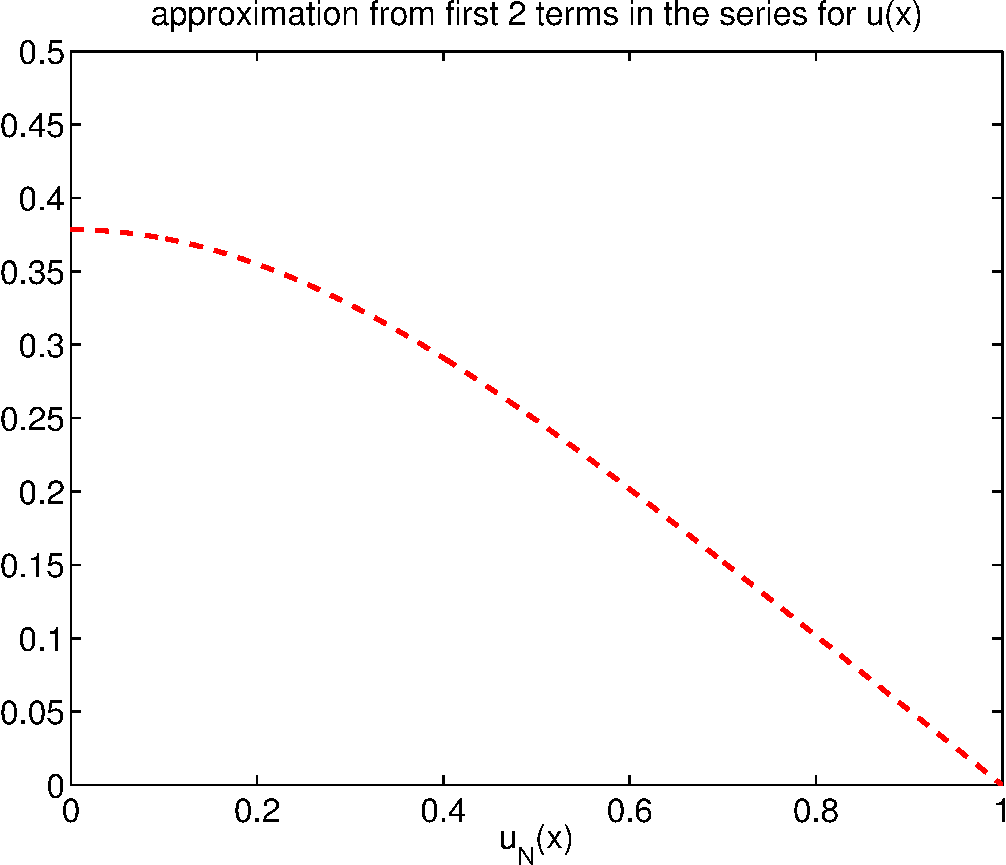
\includegraphics[scale=0.4]{bvps3_2a}

   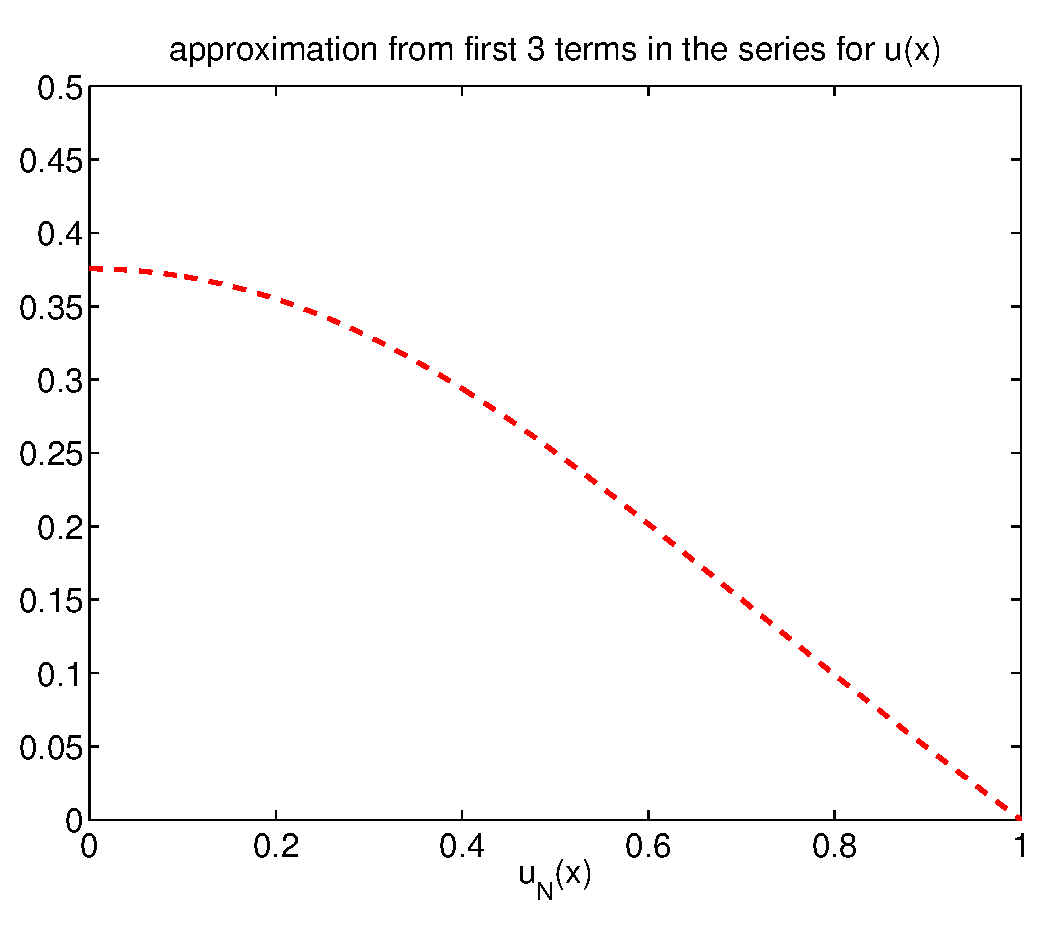
\includegraphics[scale=0.4]{bvps3_3a}\quad
   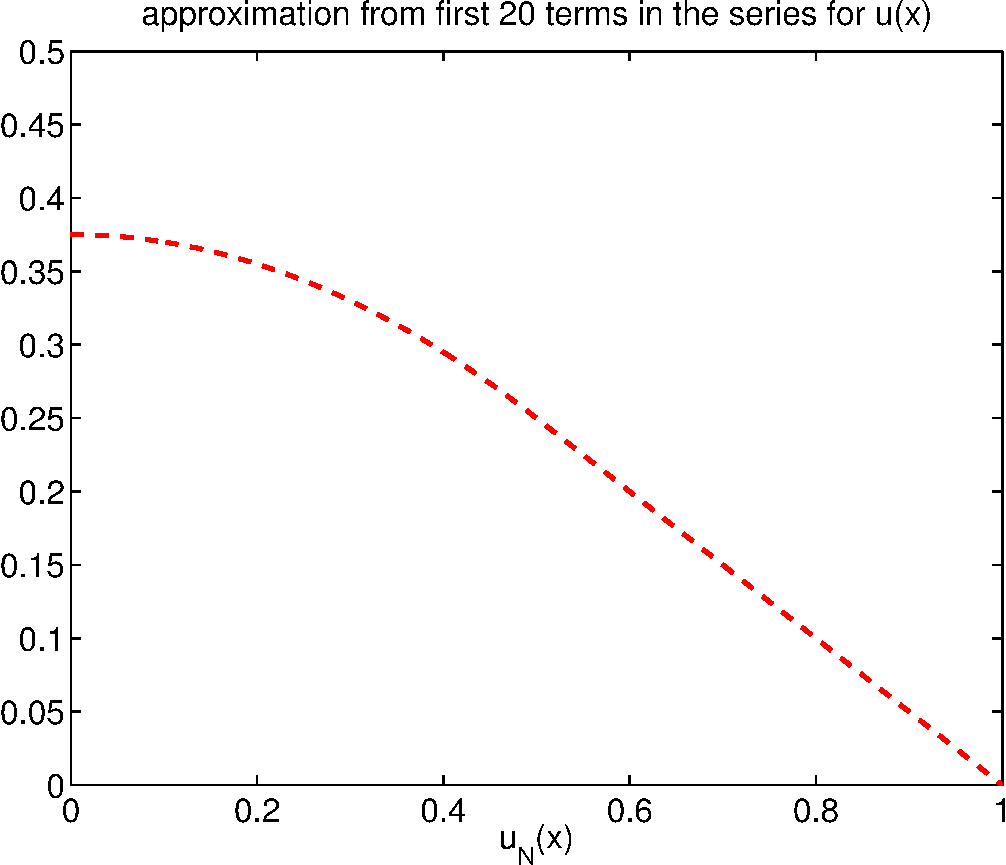
\includegraphics[scale=0.4]{bvps3_20a}
\end{center}
\input bvps_code3

\end{enumerate}
\end{solution}}{}

